\documentclass[a4paper,12pt]{book}
\usepackage[utf8]{inputenc}
\usepackage{graphicx}

\usepackage{listings}
\usepackage{color}

\definecolor{lightgray}{rgb}{0.6, 0.6, 0.6}
\definecolor{darkgray}{rgb}{0.4, 0.4, 0.4}
%\definecolor{purple}{rgb}{0.65, 0.12, 0.82}
\definecolor{editorGray}{rgb}{0.95, 0.95, 0.95}
\definecolor{editorOcher}{rgb}{1, 0.5, 0} % #FF7F00 -> rgb(239, 169, 0)
\definecolor{editorGreen}{rgb}{0, 0.5, 0} % #007C00 -> rgb(0, 124, 0)
\definecolor{orange}{rgb}{1,0.45,0.13}      
\definecolor{olive}{rgb}{0.17,0.59,0.20}
\definecolor{brown}{rgb}{0.69,0.31,0.31}
\definecolor{purple}{rgb}{0.38,0.18,0.81}
\definecolor{lightblue}{rgb}{0.1,0.57,0.7}
\definecolor{lightred}{rgb}{1,0.4,0.5}

% CSS
\lstdefinelanguage{CSS}{
	keywords={color,background-image:,margin,padding,font,weight,display,position,top,left,right,bottom,list,style,border,size,white,space,min,width, transition:, transform:, transition-property, transition-duration, transition-timing-function}, 
	sensitive=true,
	morecomment=[l]{//},
	morecomment=[s]{/*}{*/},
	morestring=[b]',
	morestring=[b]",
	alsoletter={:},
	alsodigit={-}
}

% JavaScript
\lstdefinelanguage{JavaScript} {
	morekeywords={
		break,const,continue,delete,do,while,export,for,in,function,
		if,else,import,in,instanceOf,label,let,new,return,switch,this,
		throw,try,catch,typeof,var,void,with,yield
	},
	sensitive=false,
	morecomment=[l]{//},
	morecomment=[s]{/*}{*/},
	morestring=[b]",
	morestring=[d]'
}

\lstdefinelanguage{HTML5}{
	language=html,
	sensitive=true,   
	alsoletter={<>=-},    
	morecomment=[s]{<!-}{-->},
	tag=[s],
	otherkeywords={
		% General
		>,
		% Standard tags
		<!DOCTYPE,
		</html, <html, <head, <title, </title, <style, </style, <link, </head, <meta, />,
		% body
		</body, <body,
		% Divs
		</div, <div, </div>, 
		% Paragraphs
		</p, <p, </p>,
		% scripts
		</script, <script,
		% More tags...
		<canvas, /canvas>, <svg, <rect, <animateTransform, </rect>, </svg>, <video, <source, <iframe, </iframe>, </video>, <image, </image>, <header, </header, <article, </article
	},
	ndkeywords={
		% General
		=,
		% HTML attributes
		charset=, src=, id=, width=, height=, style=, type=, rel=, href=,
		% SVG attributes
		fill=, attributeName=, begin=, dur=, from=, to=, poster=, controls=, x=, y=, repeatCount=, xlink:href=,
		% properties
		margin:, padding:, background-image:, border:, top:, left:, position:, width:, height:, margin-top:, margin-bottom:, font-size:, line-height:,
		% CSS3 properties
		transform:, -moz-transform:, -webkit-transform:,
		animation:, -webkit-animation:,
		transition:,  transition-duration:, transition-property:, transition-timing-function:,
	}
}

\lstdefinestyle{htmlcssjs} {%
	% General design
	%  backgroundcolor=\color{editorGray},
	basicstyle={\footnotesize\ttfamily},   
	frame=b,
	% line-numbers
	xleftmargin={0.75cm},
	numbers=left,
	stepnumber=1,
	firstnumber=1,
	numberfirstline=true, 
	% Code design
	identifierstyle=\color{black},
	keywordstyle=\color{blue}\bfseries,
	ndkeywordstyle=\color{editorGreen}\bfseries,
	stringstyle=\color{editorOcher}\ttfamily,
	commentstyle=\color{brown}\ttfamily,
	% Code
	language=HTML5,
	alsolanguage=JavaScript,
	alsodigit={.:;},  
	tabsize=2,
	showtabs=false,
	showspaces=false,
	showstringspaces=false,
	extendedchars=true,
	breaklines=true,
	% German umlauts
	literate=%
	{Ö}{{\"O}}1
	{Ä}{{\"A}}1
	{Ü}{{\"U}}1
	{ß}{{\ss}}1
	{ü}{{\"u}}1
	{ä}{{\"a}}1
	{ö}{{\"o}}1
}
%
\lstdefinestyle{py} {%
	language=python,
	literate=%
	*{0}{{{\color{lightred}0}}}1
	{1}{{{\color{lightred}1}}}1
	{2}{{{\color{lightred}2}}}1
	{3}{{{\color{lightred}3}}}1
	{4}{{{\color{lightred}4}}}1
	{5}{{{\color{lightred}5}}}1
	{6}{{{\color{lightred}6}}}1
	{7}{{{\color{lightred}7}}}1
	{8}{{{\color{lightred}8}}}1
	{9}{{{\color{lightred}9}}}1,
	basicstyle=\footnotesize\ttfamily, % Standardschrift
	numbers=left,               % Ort der Zeilennummern
	%numberstyle=\tiny,          % Stil der Zeilennummern
	%stepnumber=2,               % Abstand zwischen den Zeilennummern
	numbersep=5pt,              % Abstand der Nummern zum Text
	tabsize=4,                  % Groesse von Tabs
	extendedchars=true,         %
	breaklines=true,            % Zeilen werden Umgebrochen
	keywordstyle=\color{blue}\bfseries,
	frame=b,
	commentstyle=\color{brown}\itshape,
	stringstyle=\color{editorOcher}\ttfamily, % Farbe der String
	showspaces=false,           % Leerzeichen anzeigen ?
	showtabs=false,             % Tabs anzeigen ?
	xleftmargin=17pt,
	framexleftmargin=17pt,
	framexrightmargin=5pt,
	framexbottommargin=4pt,
	%backgroundcolor=\color{lightgray},
	showstringspaces=false,      % Leerzeichen in Strings anzeigen ?
}%
%
\makeatother

\begin{document}

\author{Tsiry RADIASON}
\title{Application on NodeJS, Express based on ES2015}
\date{June 2016}

\frontmatter
\maketitle
\tableofcontents

\mainmatter
% Tools
\chapter{Outils de developpement}
Nous specifierons dans cette partie les outils que nous avons employés pour nous assister dans la conception et la réalisation de notre projet.
Etant donné certaines spécifications de notre application, elle n'exige pas de grandes ressource matériels alors nous allons passer directement au ressources logiciels. Nous présenterons les caractéristiques du serveur qui héberge l'application dans la partie de la partie realisation et test.
Bien que l'outil de develloppent de base soit un éditeur de text. La partie serveur a besoin decertains outils spécialisé, de même que la partie client.

% Functions
\include{./chapters/Architecture}

% Modules
\include{./chapters/Server}
\section{Node.Js Design Pattern}
Chaque plateforme a sa propre manière de faire les choses et cela infule grandement sur l'evolution de la plateforme te de sa communauté.
Pour Node.Js certaines des principes de conception vient des inventeurs de la plateforme, des contributeurs dans la construction du noyau, des personnes les plus importantes dans la communauté Node, et d'autres hérité par la culture du JavaScript ou influencé par la \textit{philosophie Unix}.
\subsection{Coeur et Modules}
\paragraph{Coeur}
L'une des principes de Node est d'avoir le plus petit nombre de fonctionalité dans le coeur et de laisser le reste dans l'espace utilisateur. Cela a une grande impacte sur Node.Js car cela permet à la communauté de tester et d'avoir plusieurs solutions possibles au lieux d'une seule solution imposée. Ce principe engendre une evolution rapide du système, tout en enrichissant positivement la culture des divers intervenants.
\paragraph{Modules}
Les modules dont des bibliothèques de classe qui sont des extensions de Node.Js. La philosophie de Node.Js permet à des même modules mais de version différentes de cohabiter. Une fois installé \textit{localement} ou \textit{globalement} les modules sont accessibles par toutes les classes de votre application par la méthode \textit{require(...)}.
\paragraph{installation de modules}
L'installation des modules de node sefait généralement par le module \textbf{npm}, ce module a une verision déja présent dans chaque serveur Node.Js.
Il y a deux manières d'installer un module.
\begin{enumerate}
	\item localement
	\item globalement
\end{enumerate}
Bien que techniquement, il n'existe pas de différence de fonctionnement que l'on installe un module localement ou globalement. Certains modules doivent être installé globalement pour plus de liberté et assurer que l'application soit plus légère. Dans cette catégorie nous trouvons les générateurs d'applications, les compilateurs, les emulateurs, ...
Tandis que les bibliothèques specifiques, indispensable au bon fonctionnement de l'application doit être installer localement.

Les modules installé globalement utilisent la commande CLI
\begin{lstlisting}[language=bash]
	npm install -g [module_name]
\end{lstlisting}

Il y a divers manières d'installer localement les modules. Nous emploieront la technique la plus sure. Cette methode permet d'intsaller, de catégoriser et de se rappeler des modules installé. Dans les applications Node.Js il y a le ficher Package.json. Nous n'allons pas entrer dans les details mais voici un exemple de fichier de configuration d'un serveur Node.JS
\begin{lstlisting}[style=htmlcssjs]
  "dependencies": {
    "body-parser": "~1.15.1",
    "cookie-parser": "~1.4.3",
    "debug": "~2.2.0",
    "express": "~4.13.4",
    "jade": "~1.11.0",
    "jstransformer": "^1.0.0",
    "morgan": "~1.7.0",
    "pug": "^2.0.0-beta3",
    "serve-favicon": "~2.3.0"
  },
  "devDependencies": {
    "babel-eslint": "^6.1.0"
  }
\end{lstlisting}
Les \textit{dependencies} sont les modules necessaire pour le fonctionnement de l'application. Les modules catégorisé dans \textit{devDependencies} sont les modules utiles pendant la phase de developpement. Chaque module a pour argument la version exacte ou approximative à intsaller. Pour installer la dernière version \textit{stable} du module on place \textbf{"*"}
une fois le \textit{package.json} bien éditer il suffit de taper la commande CLI suivante.
\begin{lstlisting}[language=bash]
	npm install 
\end{lstlisting}
Il installera alors tous les modules inscris dans le fichier de configuration dans un dossier \textbf{node modules}
\section{Node.Js avec es6}
\subsection{Initialisation}
On commence par initialiser le ficher \textit{package.json}
\begin{lstlisting}[language=bash]
	npm init -y
\end{lstlisting}
Cela crée le fichier et introduit les valeurs par defauts tel que le non du projet qui par defaut est le nom du dossier qui le contient, la version, la description ...
On intsalle par la suite les dependances de developpement.
\begin{lstlisting}[language=bash]
	npm i -D babel-cli babel-preset-2015 nodemon
\end{lstlisting}
on configure par la suite le module \textit{Babel} avec le fihier \textbf{.babelrc} en y inscrivant les lignes suivantes:
\begin{lstlisting}[style=htmlcssjs]
{
	"presets": ["es2015"]
}
\end{lstlisting}

\subsection{Minimal server}
Une fois l'initialisation terminé on peut déja lancer un serveur minimal grace au code suivant.
\begin{lstlisting}[style=htmlcssjs]
import http from 'http';

http.createServer((req, res) => {
  res.writeHead(200, {'Content-type': "text/plain"});
  res.end("Hello world\n");
}).listen(3000, '127.0.0.1');

console.log("server running at http://127.0.0.1:3000/");
\end{lstlisting}
Ensuite on place un script qui permet de lancer le mode developpement dans \textit{package.json}:
\lstinputlisting[style=htmlcssjs, firstline=7, lastline=12]{../server/package.json}
Utiliser \textit{nodemon} permet de modifier en \textit{live} le code du serveur et sera mis à jour et redemarre automatiquement.
Le lancement \textit{build} est pour la production d'une version deployable de l'application. Pour pouvoir profiter de la version finale sans à avoir le lancer manuellement, on a le script \textit{default}

\section{Express Js}
cette section parlera d'express
\section{CRUD, Express et MongoDB}
\paragraph{CRUD}C'est un acronym pour \textbf{CREATE}, \textbf{READ}, \textbf{UPDATE} et \textbf{DELETE} dans certaines denomition il existe un dernier element \textbf{EXECUTE}. C'est une liste d'operation que l'on demande au serveur d'executer au travers des requêtes \textbf{POST}, \textbf{GET}, \textbf{PUT} et \textbf{DELETE} respectivement.
\begin{center}
	\makebox[\textwidth]{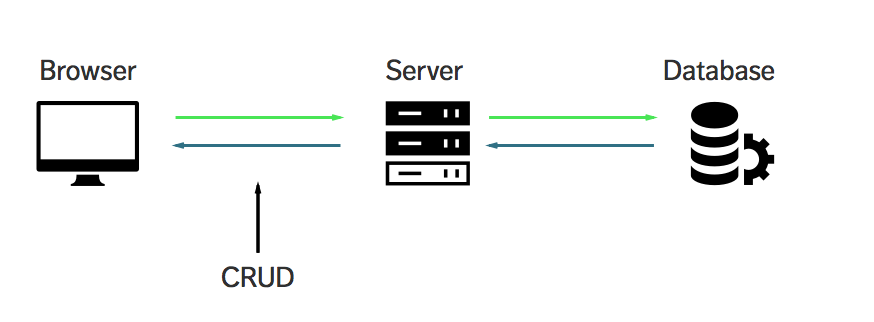
\includegraphics[width=\textwidth]{./media/crud-express-mongo.png}}
\end{center}
\subsection{}

\include{./chapters/Client}

\backmatter

% bibliography, glossary and index would go here.

\end{document}